\documentclass[lettersize,journal]{IEEEtran}
\usepackage{amsmath,amsfonts}
\usepackage{algorithmic}
\usepackage{algorithm}
\usepackage{array}
\usepackage[caption=false,font=normalsize,labelfont=sf,textfont=sf]{subfig}
\usepackage{textcomp}
\usepackage{stfloats}
\usepackage{url}
\usepackage{verbatim}
\usepackage{graphicx}
\usepackage{cite}
% \usepackage{bbold}
\usepackage{booktabs}
\usepackage{multirow}
\usepackage{colortbl}
\usepackage{adjustbox}
\usepackage{xcolor}
\newcommand{\blue}[1]{\textcolor{blue}{#1}}

% Hyperlinks (load at end of preamble)
\usepackage[hidelinks]{hyperref}
\usepackage[capitalize]{cleveref}

\hyphenation{op-tical net-works semi-conduc-tor IEEE-Xplore}
% updated with editorial comments 8/9/2021

\begin{document}

\title{NaCo: Realizing Human-Like Naturalistic Psychological Counseling with CoRA-MCTS Planning and Progressive-SimPO Alignment}

\author{Aoduo Li, Peikai Lin, Jiancheng Li, Jiahao Xian, Haoran Lv, Yihang Dong and Xuhang Chen
        % <-this % stops a space
\thanks{This work was supported by Guangdong Basic and Applied Basic Research Foundation (Grant No. 2024A1515140010).}
\thanks{Aoduo Li, Jiancheng Li, Peikai Lin, Jiahao Xian, and Haoran Lv are with the School of Advanced Manufacturing, Guangdong University of Technology, Jieyang 515200, China (e-mail: 3123009124@mail2.gdut.edu.cn; voidljc@gmail.com; pkailin@gmail.com; xianjiahao@mails.gdut.edu.cn; 3123008610@mail2.gdut.edu.cn).}
\thanks{Yihang Dong is with the Shenzhen Institutes of Advanced Technology, Chinese Academy of Sciences, Shenzhen 518055, China (e-mail: yh.dong@siat.ac.cn).}
\thanks{Xuhang Chen is with the School of Computer Science and Engineering, Huizhou University, Huizhou 516007, China (e-mail: xuhangc@hzu.edu.cn).}
\thanks{Xuhang Chen is the corresponding author.}
}

% The paper headers
\markboth{Journal of \LaTeX\ Class Files,~Vol.~14, No.~8, August~2021}%
{Shell \MakeLowercase{\textit{et al.}}: A Sample Article Using IEEEtran.cls for IEEE Journals}

% Remember, if you use this you must call \IEEEpubidadjcol in the second
% column for its text to clear the IEEEpubid mark.

\maketitle

\begin{abstract}
The proliferation of consumer electronic devices, including smartphones, smart speakers, and wearable health monitors, has created unprecedented opportunities for AI-powered mental health support accessible to everyday users.
However, current large language models (LLMs) for psychological counseling face two critical challenges: insufficient human-like qualities in training data and templated dialog generation, which severely limit their deployment in consumer-grade mental wellness applications.
In this paper, we propose NaCo (Naturalistic Counseling), a comprehensive framework combining data synthesis enhancement with model alignment optimization to improve psychological counseling quality for consumer electronics platforms.
First, we design NaCo-DS (NaCo Data Synthesis), which simulates emotional evolution of clients while incorporating the CoRA-MCTS (Chain-of-Thought and Retrieval-Augmented Monte Carlo Tree Search) strategy into the counselor agent, producing synthesized data with realistic emotional transitions, natural language flow, and professional counseling techniques suitable for edge deployment.
Second, to address multi-turn dialog alignment challenges in offline reinforcement learning, we introduce Progressive-SimPO, a turn-level preference optimization method that significantly enhances response naturalness for conversational AI applications.
We construct the NaCo-Corpus dataset and apply Progressive-SimPO training to Qwen2.5-7B-Instruct.
Experimental results demonstrate that our NaCo-Prog-SimPO model achieves superior overall scores compared with 14 mainstream LLMs on public professional test sets and significantly outperforms domain-specific models in multi-turn dialog preference win rates, making it highly suitable for integration into consumer mental health applications.
\end{abstract}

\begin{IEEEkeywords}
Psychological counseling, large language models, mental health applications, preference optimization, Monte Carlo tree search
\end{IEEEkeywords}

\section{Introduction}
\IEEEPARstart{T}{he} proliferation of consumer electronics has transformed mental health support, with smartphones and wearables becoming ubiquitous platforms for AI-powered wellness applications \cite{TCE_EdgeAI2024, TCE_SmartHome2023, TCE_VoiceAssist2023}. Despite this potential, a critical global shortage of professionals leaves approximately 75\% of those in need without adequate care. Consumer platforms, through their intimate and constant user interaction, offer a promising avenue to bridge this gap via AI-assisted psychological support systems.

However, effective AI counselors must demonstrate more than linguistic fluency; they require empathy, emotional awareness, and the strategic application of psychological knowledge \cite{Yang2024, Liu2023, Na2024}. Replicating these nuanced human qualities presents formidable challenges, as counseling involves complex temporal emotional dynamics and contextual sensitivity. 

The integration of large language models (LLMs) into consumer electronics faces significant data and optimization hurdles \cite{TCE_Wearable2024, TCE_MentalHealth2024}. Most open-source datasets are limited to single-turn Q\&A or are automatically synthesized \cite{Zhang2024a, Chen2023, Qiu2024}, failing to capture the progressive emotional evolution and adaptive interventions characteristic of real therapeutic encounters. Consequently, models trained on such data often produce mechanical responses that lack genuine rapport and professional guidance.



Furthermore, current models predominantly rely on Supervised Fine-Tuning (SFT), which promotes rigid response imitation rather than adaptive behavior \cite{Dong2024}. While Reinforcement Learning (RL) can enhance flexibility \cite{Ouyang2022}, online RL is computationally prohibitive for edge deployment, and offline methods like DPO \cite{Rafailov2023} or SimPO \cite{Meng2024} struggle with multi-turn coherence \cite{Chu2025, Singh2002}.

To address these limitations, we propose \textbf{NaCo}, a unified strategy for naturalistic counseling optimized for consumer platforms. NaCo consists of two components:
\begin{itemize}
    \item \textbf{NaCo Data Synthesis (NaCo-DS)}: Generates multi-turn dialogs with realistic emotional evolution by simulating dynamic client states and adaptive counselor interventions.
    \item \textbf{Progressive Simple Preference Optimization (Progressive-SimPO)}: Enables turn-level preference learning with contextual integration, ensuring coherent and stylistically consistent responses without the high cost of online RL.
\end{itemize}



During data generation, we introduce \textbf{CoRA-MCTS}, a Chain-of-Thought and Retrieval-Augmented Monte Carlo Tree Search framework. By integrating reasoning-based RAG \cite{Lewis2020, Gao2023} with strategic search, CoRA-MCTS allows the agent to dynamically infer client states and retrieve psychological knowledge. This dual approach yields AI counselors with the naturalness, empathy, and professional competence required for effective interaction on consumer-grade devices.
Our key contributions are: (1) an integrated NaCo framework enhancing LLMs in counseling through empathy, adaptive planning, and professional response generation; (2) NaCo-DS, a data synthesis framework simulating emotional dynamics for realistic multi-turn dialog generation; (3) CoRA-MCTS for dynamic response planning via reasoning-augmented search; and (4) Progressive-SimPO, a turn-level preference optimization method achieving natural multi-turn responses while avoiding costly online RL.

\section{Related Work}

\subsection{Data Synthesis for Psychological Counseling}
Existing counseling synthesis methods lack diversity and controllability. SMILE \cite{Qiu2024} expands single-turn data via ChatGPT but lacks emotional coherence mechanisms. CPsyCoun \cite{Zhang2024a} reconstructs dialogues from notes but misses the interplay between emotional trajectory and adaptive interventions. PsyDT \cite{Xie2024} employs GPT-4 digital twins but is cost-prohibitive. These methods produce linguistically correct but functionally stagnant conversations and do not model the counselor's reasoning---the \textit{why} behind strategic choices. NaCo-DS addresses this by explicitly simulating emotional dynamics and strategic adaptations.

\subsection{Linguistics-aware Reasoning and External Knowledge}
MCTS has emerged as a powerful paradigm for planning in LLMs \cite{Hao2023, Zhang2024b}, excelling in reasoning tasks (CoAT \cite{Pan2025}, rStar \cite{Qi2024}). RAG is vital for factuality \cite{Lewis2020, Gao2023, Asai2023}, though standard RAG struggles with psychological query ambiguity. Recent works like MCTS-RAG \cite{Hu2025} combine these by formulating retrieval-generation as an MDP \cite{Wang2024, Browne2012}. Unlike math-oriented search relying on binary correctness, NaCo-DS introduces a multi-dimensional psychological reward function, enabling the counselor agent to balance empathy, professional depth, and stylistic consistency.

\subsection{Preference Optimization for Multi-Turn Dialogues}
DPO \cite{Rafailov2023} and SimPO \cite{Meng2024} are standard offline preference methods. Step-DPO \cite{Lai2024} adds step-level supervision, while SDPO \cite{Kong2025} proposes segment-level optimization, but neither fully leverages turn-by-turn history. Incorporating entire histories into a single objective causes overfitting to superficial patterns \cite{Singh2002}, and online RL \cite{Ouyang2022} remains impractical for edge deployment. Our Progressive-SimPO bridges this gap with a turn-level, reference-free objective maintaining temporal coherence.
\section{Methodology}

The NaCo framework simulates realistic multi-turn consultations and generates emotionally natural dialogues as the foundation for Progressive-SimPO optimization. It comprises three core innovations: persona-persistent data synthesis, reasoning-augmented MCTS planning, and progressive turn-level alignment. \blue{The overall architecture is illustrated in \cref{fig:framework}.}

\begin{figure*}[htbp]
    \centering
    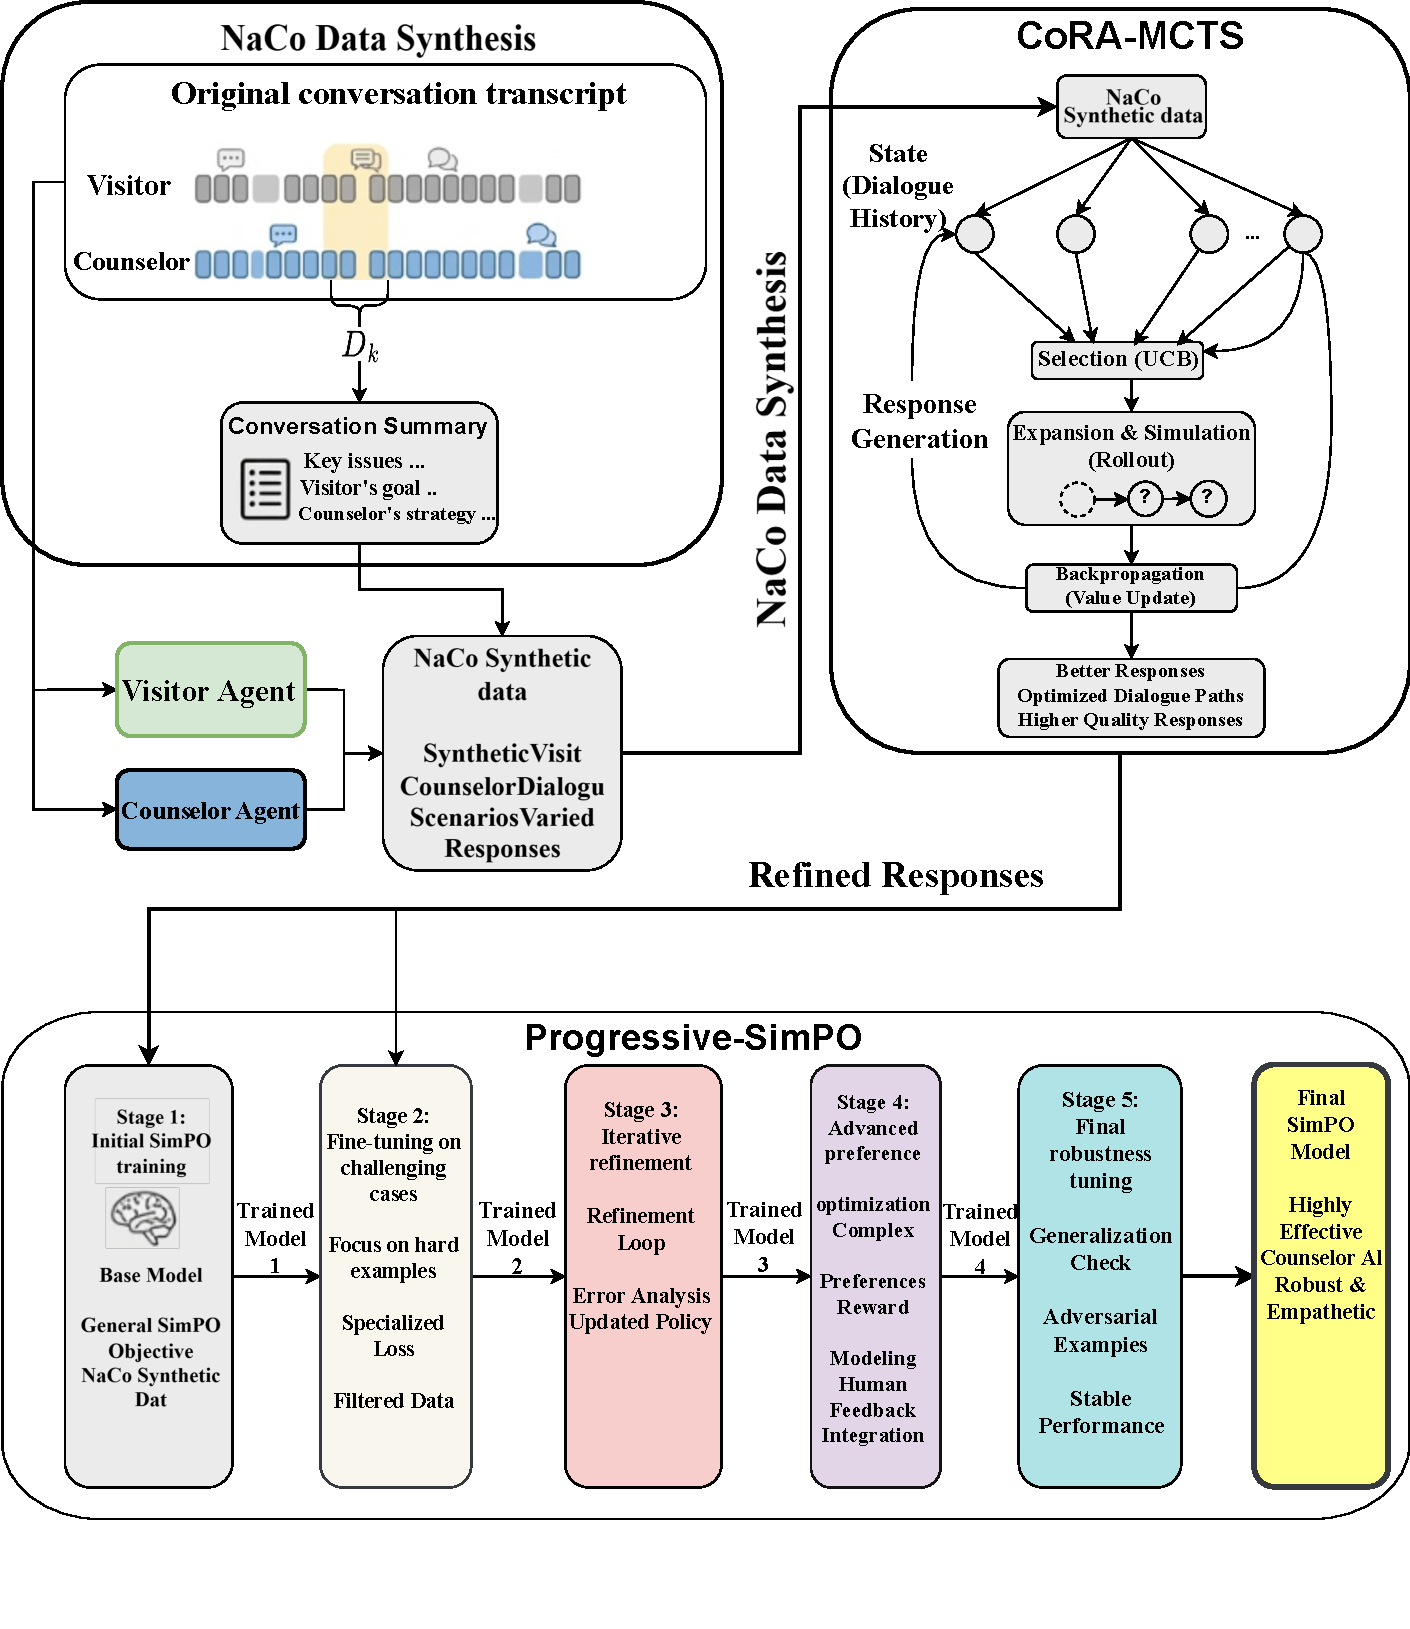
\includegraphics[width=\linewidth]{images/architecture_v2.pdf}
    \caption{\blue{The overall architecture of the NaCo framework. It consists of three stages: (1) NaCo-DS for persona-persistent data synthesis, (2) CoRA-MCTS for reasoning-augmented planning, and (3) Progressive-SimPO for turn-level alignment.}}
    \label{fig:framework}
\end{figure*}

\subsection{NaCo Data Synthesis (NaCo-DS)}
The synthesis process aims to transform static case records into dynamic, interactive sessions. This requires the client agent and the counselor agent to maintain a high degree of role-playing consistency and technical depth.

\blue{Unlike prior methods (SMILE, CPsyCoun, PsyDT) that merely rewrite input data or employ static templates, NaCo-DS fundamentally restructures the generation process by introducing a search-based planning loop. The persistent persona context enables emotional trajectory simulation across turns, which is a generative mechanism rather than simple input preprocessing. Combined with CoRA-MCTS's multi-dimensional therapeutic evaluation, NaCo-DS transforms static case records into dynamically adaptive sessions that model both the ``what'' and ``why'' of counselor decisions.}

\subsubsection{Client Personality and Emotional Trajectory}
Unlike traditional synthesis that focuses only on "matching" the input report, NaCo-DS extracts a persistent persona context that guides the client agent's responses throughout the session. This ensures that the client's emotional fluctuations follow a logical progression (e.g., from initial defensive reticence to eventual vulnerability).
Let the original reference chat history (or case report) be
\begin{equation}
H_{all} = \{D_{1}, D_{2}, \dots , D_{n}\},
\end{equation}
where $D_{i}$ represents one turn of dialogue containing both client and therapist information. 
The client agent first constructs a summary of its own hidden state, denoted as:
\begin{equation}
P = f_{\text{sum}}(H_{all}) \oplus E_{init},
\end{equation}
where $f_{\text{sum}}$ is the summarization function, $E_{init}$ represents the initial emotional state, and $\oplus$ denotes the concatenation of personality traits, core stressors, and specific communication quirks. This persistent context $P$ is prepended to the system prompt in every turn to maintain "in-character" consistency.

\subsubsection{Agent Interaction-based Simulation}
The dialogue proceeds as a sequence of interactions between the Consultant agent and the Visitor agent. Let the set of synthesized dialogue history up to turn $k-1$ be:
\begin{equation}
H_{k} = \{\mathbf{t}_{1}, \mathbf{t}_{2}, \dots , \mathbf{t}_{k - 1}\},
\end{equation}
where $\mathbf{t}_i = (\mathbf{t}_{i}^{C}, \mathbf{t}_{i}^{V})$ denotes the synthesized response pair. 
For each new turn $k$, we aim to generate a high-quality pair $\mathbf{t}_k$ that mimics the professional intent of the reference dialogue $D_k = (D_k^C, D_k^V)$ while exhibiting the naturalistic flow of a real-time conversation.
Numerical simulations and user feedback indicate that purely imitation-based synthesis (Simple-SFT) often ignores the underlying reasoning behind a counselor's choice. To solve this, we incorporate the CoRA-MCTS strategy into the generation of $\mathbf{t}_k^C$.

\subsubsection{Client Agent Response Generation} The client (Visitor) agent generates its response at turn $k$ by leveraging three sources of information.
The generation process is defined as:
\begin{equation}
\mathbf{t}_{k}^{V} = f_{\text{rewrite}}^{V}(P, H_{k}, D_{k}^{V}),
\end{equation}
where $f_{\text{rewrite}}^{V}$ is the response generation function for the client agent.

\subsubsection{Counselor Agent Response Generation} The counselor agent generates its response at turn $k$ based on:
\begin{equation}
m \in \{E, X, N, S\},
\end{equation}
$m$ represents the collection of the counselor agent's reply strategies, where $E$ stands for empathic support, $X$ for exploratory guidance, $N$ for neutral verbalization, and $S$ for silent listening.
Depending on the value of $m$, the generation process may also incorporate information from a Retrieval-Augmented Generation (RAG) module:
\begin{equation}
\mathbf{t}_{k}^{C} = \begin{cases} f_{\text{rewrite}}^{C}(H_{k}, D_{k}, m, f_{\text{RAG}}(H_{k}, D_{k}^{V})) & m \in \{E, X\} \\ f_{\text{rewrite}}^{C}(H_{k}, D_{k}, m) & m \in \{N, S\} \end{cases}
\end{equation}
where $f_{\text{rewrite}}^{C}$ is the counselor agent's response generation function, and $f_{\text{RAG}}(H_k, D_k^V)$ is the output of the RAG module.

\blue{The retrieval corpus comprises three sources: (1) 2,450 professional counseling technique descriptions from 12 authoritative psychology textbooks covering CBT, DBT, Person-Centered Therapy, and Motivational Interviewing; (2) 1,200 curated case vignettes from PsyDTCorpus with expert annotations; and (3) 380 crisis intervention protocols from national hotline guidelines. All entries were reviewed by two licensed counselors. The corpus is indexed via dense passage retrieval with periodic review, and harmful or outdated content is flagged through keyword filters and manual audit with provenance metadata.}

\subsection{CoRA-MCTS: Reasoning-Augmented Planning}
For the counselor agent, we use CoRA-MCTS to explore multiple synthesis candidates and select optimal responses. This approach mimics the clinical reasoning of a human therapist who balances several potential interpretations before speaking.
The node state in the search tree is defined as:
\begin{equation}
s = \langle H_{k}, \mathbf{t}_k^V, m, d \rangle,
\end{equation}
where $H_{k}$ represents the synthesized history, $\mathbf{t}_k^V$ is the client's current query, $m$ denotes the candidate response strategy, and $d$ is the search depth.

\subsubsection{Heuristic Reward Function}
To guide the tree search toward high-quality counseling, we employ a multi-dimensional reward function $R$. We use an LLM-as-a-judge to score generated candidates on a scale of 1-5 across four critical therapeutic dimensions:
\begin{itemize}
    \item \textbf{Empathy ($r_e$):} The degree of emotional validation and warmth.
    \item \textbf{Professionalism ($r_p$):} The adherence to psychological intervention protocols (e.g., CBT, DBT).
    \item \textbf{Exploration ($r_x$):} The ability to prompt the client for deeper self-reflection.
    \item \textbf{Safety ($r_s$):} A strict check to avoid harmful or non-professional advice.
\end{itemize}
\blue{The 5-point Likert scale is widely adopted in psychological assessment instruments (e.g., PHQ-9, GAD-7) and LLM evaluation benchmarks~\cite{Zheng2024}, providing sufficient discriminative power while maintaining reliability for LLM-as-judge scoring.}
The final reward is calculated as $R = f_{\text{reward}}(r_e, r_p, r_x, r_s)$. By maximizing this reward, the agent learns to synthesize dialogues that are not just fluent, but clinically meaningful.

\blue{The LLM-based reward function captures nuanced multi-dimensional quality (empathy, professionalism, exploration, safety) that simple rule-based heuristics (e.g., keyword matching, sentiment scoring) cannot decompose. We note that this computational cost is incurred only during offline data synthesis, not during inference. On 8$\times$A100 GPUs, reward computation averages 2.3 seconds per candidate, with the full NaCo-Corpus synthesis (6,098 sessions) requiring approximately 180 GPU-hours.}

\subsubsection{Strategic Selection and Backpropagation}
Selection follows the Upper Confidence Bound for Trees (UCT) criterion:
\begin{equation}
\label{eq:uct}
\operatorname{UCT}(s') = \frac{Q(s')}{N(s')} + c \sqrt{\frac{\ln N(s)}{N(s')}},
\end{equation}
where $Q(s')$ is the cumulative reward, $N(s')$ is the visit count, and $c$ is the exploration constant ($c=1$). 
At each node, the agent expands $K$ potential response strategies. For each strategy, a reasoning chain (Chain-of-Thought) and retrieval results (RAG) are generated to produce a candidate response. After reaching a leaf node (simulation), the reward is backpropagated to update the visit counts and accumulated rewards of all parent nodes. The final synthesized response $t_k^C$ is the branch with the highest visit count and reward density.

\begin{algorithm}[H]
\caption{CoRA-MCTS for Counselor Agency}
\label{alg:mcts}
\begin{algorithmic}[1]
\STATE \textbf{Input:} History $H_k$, Query $q_k$, Iterations $T$
\STATE \textbf{Output:} Optimal Response $y^*$
\STATE Initialize root node $s_0 \leftarrow \langle H_k, q_k, \text{depth}=0 \rangle$
\FOR{$t=1$ to $T$}
    \STATE $s_{leaf} \leftarrow \text{Selection}(s_0)$ utilizing \cref{eq:uct}
    \IF{$s_{leaf}.N > N_{thr}$}
        \STATE $\mathcal{S} \leftarrow \text{Expansion}(s_{leaf})$ // Generate strategies
        \STATE $y_{cand} \leftarrow \text{LLM}(s_{leaf}.context, \mathcal{S})$
        \STATE $s_{leaf} \leftarrow \text{Append}(s_{leaf}, y_{cand})$
    \ENDIF
    \STATE $R \leftarrow \text{Scorer}(s_{leaf}.y)$ // Heuristic Scorer
    \STATE $\text{Backpropagate}(s_{leaf}, R)$
\ENDFOR
\STATE \RETURN $y^* = \arg\max_{child \in s_0} Q(child)/N(child)$
\end{algorithmic}
\end{algorithm}

\subsection{Progressive-SimPO Alignment}

\subsubsection{Multi-Turn Preference Contradictions}
Standard offline methods (DPO, SimPO) struggle with multi-turn dialogues due to the ``Credit Assignment Problem'': when a whole conversation is labeled as a single sample, conflicting turn-level quality causes \textbf{gradient diffusion} (good behaviors diluted by average turns) and \textbf{gradient imbalance} (over-penalizing negatives while under-rewarding positives).

\subsubsection{Temporal Unfolding and Formalization}
Progressive-SimPO resolves these issues by unfolding the multi-turn session into $N-1$ turn-level preference pairs. For each turn $i \geq 2$, we define the context $\mathbf{x}_i$ as the concatenation of all previous turns and the current query.
The implicit reward for a response $y$ is:
\begin{equation}
\label{eq:implicit_reward}
r(\mathbf{x}_{i}, y) = \beta \cdot \frac{1}{|y|} \log \pi_{\theta}(y \mid \mathbf{x}_{i}),
\end{equation}
where $|y|$ is the token length. Length normalization is crucial to prevent "verbosity hacking," where the model generates longer, fluffier responses to artificially inflate log-likelihood.
The preference probability between the RA-MCTS generated response $y_i^+$ and the base model's response $y_i^-$ follows the Bradley-Terry model with an introduced margin $\gamma$:
\begin{equation}
\label{eq:sigmoid_prob}
p(y^{+} \succ y^{-} \mid x) = \sigma(r(x, y^{+}) - r(x, y^{-}) - \gamma).
\end{equation}
The margin $\gamma > 0$ ensures that the model learns a clear distinction between professional counseling techniques and generic AI replies.

During training, maximizing the log probability of \cref{eq:sigmoid_prob} is equivalent to minimizing its negative log probability:
\begin{equation}
\label{eq:loss_single}
\mathcal{L}_{i}(\theta) = -\log \sigma(r(\mathbf{x}_{i}, y_{i}^{+}) - r(\mathbf{x}_{i}, y_{i}^{-}) - \gamma).
\end{equation}

Substituting \cref{eq:implicit_reward} into \cref{eq:loss_single}, the objective function for Progressive-SimPO for each turn $i$ ($i = 2,3,\dots ,N$) can be expressed as:
\begin{multline}
\mathcal{L}_{i}(\theta) = -\log \sigma \left(\beta \frac{1}{|y_{i}^{+}|} \log \pi_{\theta}(y_{i}^{+} \mid x_{i}) \right. \\
\left. - \beta \frac{1}{|y_{i}^{-}|} \log \pi_{\theta}(y_{i}^{-} \mid x_{i}) - \gamma\right).
\end{multline}

Taking the arithmetic mean over the $(N-1)$ steps of the same conversation yields the global objective of Progressive-SimPO:
\begin{equation}
\mathcal{L}_{\text{Prog-SimPO}}(\theta) = \frac{1}{N - 1} \sum_{i = 2}^{N} \mathcal{L}_{i}(\theta).
\end{equation}

% The final objective function of Progressive-SimPO is given in Appendix A.1.
This design ensures that the gradients originate only from the current response, thereby effectively reducing noise;
at the same time, by relying on summation across steps, it still maintains alignment with the overall preferences of the entire dialog.

\blue{We clarify that $\beta$ serves exclusively as a reward scaling factor controlling the sharpness of the implicit reward signal, following the SimPO formulation. Unlike DPO, Progressive-SimPO is \textbf{reference-free}---there is no explicit KL divergence regularizer against a reference policy $\pi_{\text{ref}}$. Regularization against catastrophic forgetting is implicitly provided by the length-normalized log-probability formulation and the progressive turn-level decomposition, which constrains each update to a single turn's response.}

\section{Experimental Setup}

\subsection{Datasets and Topic Distribution}
We collaborated with a provincial-level hospital's psychological counseling hotline to create a proprietary dataset based on authentic, anonymized telephone recordings. This raw data comprises 2,978 multi-turn sessions across diverse demographics. Additionally, we integrated 3,120 high-quality instances from the PsyDTCorpus. 
Subsequently, we employed the NaCo-DS framework with CoRA-MCTS to resynthesize the combined data, creating the NaCo-Corpus. This synthetic but clinically-grounded dataset contains 6,098 multi-turn counseling dialogues. The conversations cover 15 major topics, including workplace stress (18\%), relationship issues (22\%), adolescent development (12\%), and mild depressive symptoms (15\%), ensuring the model generalizes across common consumer mental health scenarios as shown in \cref{fig:naco-corpus-topics}.
Furthermore, we reformatted the NaCo-Corpus into 18,294 preference pairs, using Qwen-2.5-7B-Instruct to generate rejection samples specifically designed for Progressive-SimPO training.

\blue{The hotline dataset was collected under ethical review by Guangdong University of Technology's research ethics committee. All recordings were transcribed and de-identified via a three-stage pipeline: (1) automatic PII detection using NER models targeting names, locations, phone numbers, and institutional affiliations; (2) manual review by two trained annotators; (3) secondary audit by a data governance officer. All identifiable information was replaced with category-consistent pseudonyms (e.g., ``[Name-A],'' ``[City-B]''). The study complies with China's Personal Information Protection Law (PIPL), and participants provided informed consent for research use of anonymized transcripts.}

\subsection{Evaluation Metrics}
We employ: (1) \textbf{Syntactic Metrics} (ROUGE-1/2/L, BLEU-4); (2) \textbf{BERTScore} ($F_{BERT}$); (3) \textbf{CPsyCounE} for Comprehensiveness, Professionalism, Authenticity, Safety; and (4) \textbf{Win-Rate} via GPT-4o and DeepSeek-V3 judges plus professional counselor scoring.

\begin{figure}[htbp]
    \centering
    \subfloat[Win Rate comparison]{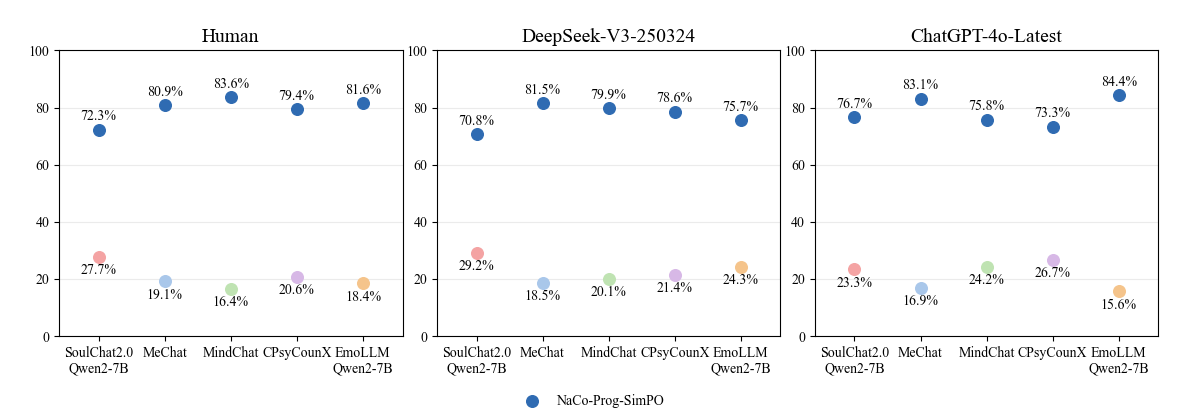
\includegraphics[width=\columnwidth]{images/fig2_0.png}\label{fig:win-rate-merged}}\\
    \subfloat[NaCo Corpus topic distribution]{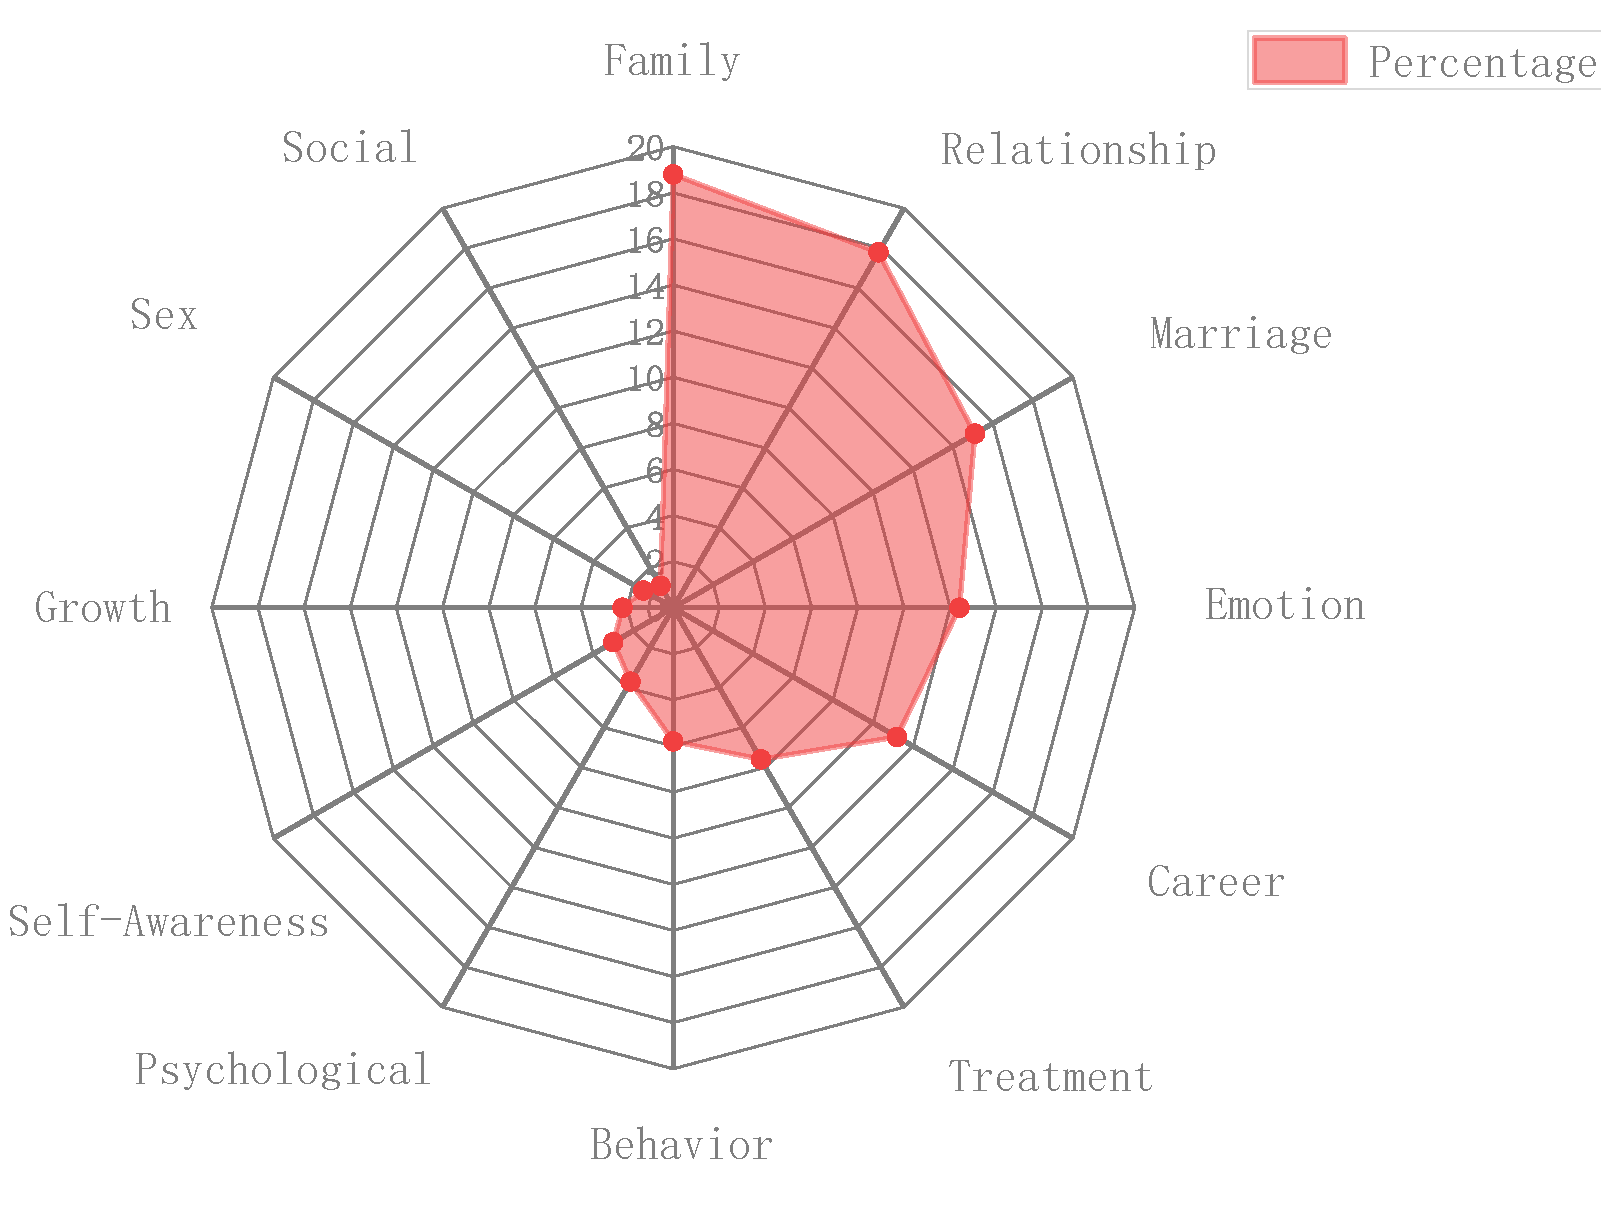
\includegraphics[width=\columnwidth]{images/fig3_0(1).pdf}\label{fig:naco-corpus-topics}}
    \caption{(a) Win Rate comparison across models and (b) NaCo Corpus topic distribution.}
    \label{fig:win-rate-topics}
\end{figure}

\subsection{Baselines}
We compare against: \textbf{Large models} (ChatGPT-4o, DeepSeek-V3), \textbf{Small models} (GLM4-9B-Chat, InternLM2-Chat-7B, Llama3/3.1-8B-Instruct, Qwen2/2.5-7B-Instruct, InternLM3-8B), and \textbf{Domain-specific} (SoulChat2.0, MeChat, MindChat, CPsyCounX, EmoLLM). Open-source models are uniformly 7B--9B scale for fair comparison.

\subsection{Implementation Details}
We use Qwen2.5-7B-Instruct as the base model, trained via LLaMAFactory for 3 epochs on 8$\times$A100 GPUs (batch size 2/GPU, Flash-attention 2, cosine scheduler with $lr=5\text{e-}05$, 32k context, FP16, AdamW, DeepSpeed3). Progressive-SimPO uses $\beta=0.1$; the same progressive method was applied to DPO for comparison.

\blue{
\begin{table}[h]
\centering
\caption{CoRA-MCTS Hyperparameters}
\label{tab:mcts_params}
\begin{tabular}{lcc}
\toprule
Parameter & Symbol & Value \\
\midrule
Branching factor & $K$ & 4 \\
Simulations & $T$ & 8 \\
Max depth & $d$ & 3 \\
Exploration constant & $c$ & 1.0 \\
Expansion threshold & $N_{thr}$ & 2 \\
Sampling temperature & -- & 0.7 \\
\bottomrule
\end{tabular}
\end{table}
CoRA-MCTS synthesis averages 4.6 seconds per counselor turn ($K \times T = 32$ LLM calls per turn). Full NaCo-Corpus synthesis (6,098 sessions) required approximately 180 GPU-hours on 8$\times$A100. At inference time, the deployed model does \textbf{not} use MCTS---it runs as a standard autoregressive model with negligible overhead.
}

\section{Evaluation}

We evaluate both human subjective preferences (Win-Rate) and semantic alignment on PsyDT and CPsyCoun benchmarks. Bold numbers indicate best performance.

\subsection{Win Rate}
We split NaCo-Corpus into train/test sets and employ LLM-as-a-Judge (DeepSeek-V3, GPT-4o) plus three volunteers and one professional counselor for win rate evaluation. \Cref{fig:win-rate-merged} shows NaCo-Prog-SimPO achieves a significant win-rate advantage.

\blue{To verify stability, we repeated each LLM-judge evaluation three times with temperature=0 and observed a mean variance of $<$2\% across runs. We evaluated $N$=120 multi-turn conversations comprising 840 total turns. The use of two independent LLM judges (GPT-4o and DeepSeek-V3) plus human evaluation serves as cross-validation. Inter-rater reliability yielded Cohen's $\kappa=0.72$ (volunteer pairwise) and $\kappa=0.78$ (volunteers vs.\ counselor), indicating substantial agreement. Human-LLM judge correlation (Spearman's $\rho$) was 0.81 (GPT-4o) and 0.76 (DeepSeek-V3).}

\begin{table}[htbp]
\centering
\caption{PsyDT Evaluation}
\label{tab:psydt}
\vskip 0.12in
\resizebox{\columnwidth}{!}{
\begin{tabular}{lllllll}
\toprule
Type & Models & R-1 & R-2 & R-L & B-4 & FBERT \\
\midrule
\multirow{2}{*}{Large} & GPT-4o & 34.45 & 7.43 & 26.21 & 1.89 & 90.03 \\
& Deepseek-V3 & 35.17 & 8.46 & 27.49 & 3.80 & 91.71 \\
\midrule
\multirow{7}{*}{Small} & GLM4-9B-Chat & 23.38 & 5.45 & 14.35 & 3.84 & 96.58 \\
& InternLM2-Chat-7B & 27.15 & 5.87 & 20.38 & 5.49 & 96.62 \\
& Llama3-8B-Instruct & 26.31 & 5.25 & 19.64 & 5.11 & 95.16 \\
& Llama3.1-8B-Instruct & 30.20 & 5.84 & 22.88 & 5.96 & 96.54 \\
& Qwen2-7B-Instruct & 23.42 & 5.28 & 15.42 & 4.05 & 96.64 \\
& Qwen2.5-7B-Instruct & 33.91 & 7.94 & 25.62 & 2.79 & 96.67 \\
& Internlm3\_8B\_instruct & 32.82 & 6.34 & 26.80 & 2.17 & 96.49 \\
\midrule
\multirow{5}{*}{Domain} & SoulChat2.0-Qwen2-7B & 36.03 & 10.88 & 28.86 & 9.99 & 96.79 \\
& MeChat & 30.71 & 7.05 & 24.43 & 6.73 & 96.55 \\
& MindChat & 22.55 & 3.44 & 17.75 & 3.48 & 93.89 \\
& CPsyCounX & 23.71 & 4.32 & 17.59 & 3.59 & 95.46 \\
& EmoLLM-Qwen2-7B-Instruct & 36.01 & 8.53 & 28.12 & 2.65 & 96.44 \\
\midrule
\multirow{5}{*}{Ours} & NaCo-FFT & 33.27 & 7.52 & 28.96 & 8.71 & 96.20 \\
& NaCo-DPO & 30.57 & 7.33 & 27.84 & 7.96 & 95.38 \\
& NaCo-SimPO & 31.26 & 7.31 & 27.71 & 7.88 & 95.42 \\
& NaCo-Prog-DPO & 34.34 & 9.66 & 28.39 & 10.23 & 96.54 \\
& \textbf{NaCo-Prog-SimPO} & \textbf{35.25} & \textbf{10.95} & \textbf{29.21} & \textbf{17.23} & \textbf{96.72} \\ 
\bottomrule
\end{tabular}
}
\end{table}

To control variables, each turn's counselor output is evaluated within the same dialog context, with the judge model labeling responses as ``chosen'' or ``reject.'' The per-turn score $s_{i,x} = \sum_{d \in D} w_d \cdot g(b_i, x)$ aggregates weighted dimension scores, where $g(b_i, x)=0.2$ if model $x$ wins turn $i$, $0.1$ for a tie, and $0$ otherwise. The overall Win Rate is $W_x = \frac{100}{N}\sum_{i=1}^{N} s_{i,x}$, converting average scores to percentages across $N$ samples.

\subsection{PsyDT Evaluation}
We evaluate 240 PsyDTCorpus test samples using ROUGE-1/2/L, BLEU-4, and $F_{BERT}$. As shown in \cref{tab:psydt}, NaCo-Prog-SimPO achieves the highest scores in ROUGE-2 (10.95), ROUGE-L (29.21), and BLEU-4 (17.23), reflecting retention of professional keywords and natural therapeutic flow.

\blue{The substantial BLEU-4 improvement (17.23 vs.\ 9.99 of SoulChat2.0) directly reflects CoRA-MCTS's ability to generate responses preserving professional counseling keywords from the retrieval corpus. The ROUGE-L gain indicates that Progressive-SimPO's turn-level optimization maintains coherent long-range textual structure, unlike session-level DPO which dilutes per-turn signals (NaCo-DPO: 27.84 vs.\ NaCo-Prog-SimPO: 29.21).}

\subsection{CPsyCoun Multi-turn Evaluation}
Using CPsyCounE, we decompose multi-turn dialogs into single-turn units evaluated with full context by GPT-4o and DeepSeek-V3 across Comprehensiveness, Professionalism, Authenticity, and Safety. As shown in \cref{tab:cpsycoun}, NaCo-Prog-SimPO achieves the highest scores, particularly in Professionalism and Authenticity.

\blue{The Professionalism and Authenticity gains (2.95/2.93 by GPT-4o judge) are attributable to CoRA-MCTS's multi-dimensional reward that explicitly optimizes for these dimensions during data synthesis. The consistent Safety score of 1.0 validates the safety reward dimension $r_s$ in the heuristic function.}

\begin{table}[ht]
\centering
\caption{CPsyCoun Evaluation Results}
\label{tab:cpsycoun}
\adjustbox{width=\linewidth}{
\begin{tabular}{llcccccccc}
\toprule
\multirow{2}{*}{Type} & \multirow{2}{*}{Models} & \multicolumn{4}{c}{GPT-4o} & \multicolumn{4}{c}{DeepSeek-V3} \\ 
& & Comp & Prof & Auth & Safety & Comp & Prof & Auth & Safety \\ 
\midrule
\multirow{2}{*}{Large} & GPT-4o & 1.91 & 2.83 & 2.82 & 1.0 & 1.92 & 2.85 & 2.81 & 0.99 \\ 
& Deepseek-V3 & 1.93 & 2.84 & 2.87 & 1.0 & 1.93 & 2.87 & 2.82 & 1.0 \\ 
\midrule
\multirow{7}{*}{Small} & GLM4-9B-Chat & 1.84 & 2.58 & 2.65 & 1.0 & 1.36 & 2.24 & 2.12 & 0.96 \\ 
& InternLM2-Chat-7B & 1.84 & 2.33 & 1.84 & 1.0 & 1.47 & 2.27 & 2.11 & 0.99 \\ 
& Llama3-8B-Instruct & 1.81 & 2.54 & 2.63 & 1.0 & 1.53 & 2.41 & 2.40 & 0.97 \\ 
& Llama3.1-8B-Instruct & 1.82 & 2.44 & 2.52 & 1.0 & 1.23 & 2.36 & 2.36 & 0.95 \\ 
& Qwen2-7B-Instruct & 1.88 & 2.78 & 2.83 & 1.0 & 1.64 & 2.56 & 2.55 & 0.92 \\ 
& Qwen2.5-7B-Instruct & 1.92 & 2.82 & 2.87 & 1.0 & 1.69 & 2.63 & 2.56 & 1.0 \\ 
& Internlm3\_8B\_instruct & 1.94 & 2.81 & 2.91 & 1.0 & 1.88 & 2.76 & 2.81 & 1.0 \\ 
\midrule
\multirow{5}{*}{Domain} & SoulChat2.0-Qwen2-7B & 1.90 & 2.68 & 2.82 & 1.0 & 1.74 & 2.51 & 2.77 & 1.0 \\ 
& MeChat & 1.38 & 1.57 & 1.59 & 0.96 & 1.46 & 1.91 & 2.19 & 0.94 \\ 
& MindChat & 1.56 & 2.26 & 2.33 & 1.0 & 1.47 & 2.06 & 2.32 & 0.99 \\ 
& CPsyCounX & 1.98 & 2.88 & 2.83 & 1.00 & 1.97 & 2.74 & 2.72 & 1.00 \\ 
& EmoLLM-Qwen2-7B-Instruct & 1.93 & 2.92 & 2.89 & 1.0 & 1.94 & 2.89 & 2.86 & 1.00 \\ 
\midrule
\multirow{5}{*}{Ours} & NaCo-FFT & 1.92 & 2.87 & 2.86 & 1.0 & 1.88 & 2.85 & 2.78 & 1.0 \\ 
& NaCo-DPO & 1.88 & 2.63 & 2.75 & 1.0 & 1.86 & 2.77 & 2.68 & 1.0 \\ 
& NaCo-SimPO & 1.87 & 2.65 & 2.77 & 1.0 & 1.83 & 2.74 & 2.71 & 1.0 \\ 
& NaCo-Prog-DPO & 1.92 & 2.89 & 2.88 & 1.0 & 1.89 & 2.88 & 2.78 & 1.0 \\ 
& \textbf{NaCo-Prog-SimPO} & \textbf{1.95} & \textbf{2.95} & \textbf{2.93} & \textbf{1.0} & \textbf{1.89} & \textbf{2.96} & \textbf{2.85} & \textbf{1.0} \\ 
\bottomrule
\end{tabular}}
\end{table}
We present a case study (\cref{tab:case_study}) comparing NaCo-Prog-SimPO with Qwen2.5-7B-Instruct on a career anxiety scenario.

\begin{table}[htbp]
\centering
\caption{Comparative Multi-turn Case Study Analysis}
\label{tab:case_study}
\resizebox{\columnwidth}{!}{
\begin{tabular}{llp{0.55\columnwidth}}
\toprule
\textbf{Turn} & \textbf{Model} & \textbf{Dialogue Content} \\
\midrule
T1 & User & "I feel like I'm never doing enough at work. Even when I finish a project, I just worry about the next one. It's like I'm on a treadmill I can't stop." \\
\cmidrule{2-3}
& NaCo & \textit{[Reflection]} "It sounds like there’s a persistent weight on you, where the 'relief' of finishing a task is immediately replaced by 'dread' for the future. You're describing a state of exhaustion where accomplishment brings no peace." \\
\midrule
T2 & User & "Exactly. My boss says I'm doing great, but I feel like a fraud. I'm just waiting for them to realize I don't know what I'm doing." \\
\cmidrule{2-3}
& Qwen2.5 & \textit{[Advice]} "You should try to make a list of your achievements. It's important to take breaks and practice deep breathing. Have you tried talking to your boss about your impostor syndrome?" \\
\cmidrule{2-3}
& NaCo & \textit{[Validation]} "That sense of being a 'fraud'—the Imposter Phenomenon—is incredibly draining, especially when your internal reality contradicts the external feedback. \textit{Probing:} To help me understand, when you hear that voice saying you're a fraud, does it sound like your own voice, or someone else's expectations?" \\
\midrule
T3 & User & "It sounds like my father. He always said that second place is the first loser. I guess I've just carried that with me into my office." \\
\cmidrule{2-3}
& NaCo & \textit{[Interpretation]} "It seems that 'treadmill' you mentioned isn't just about the current workload, but a lifelong pursuit of a standard that was never meant to be satisfied. By connecting this to your father's words, we can start to see that this pressure is an inherited script, not a reflection of your actual competence." \\
\bottomrule
\end{tabular}
}
\end{table}

As shown in \cref{tab:case_study}, the base model immediately pivots to generic advice, while NaCo-Prog-SimPO employs professional strategies: emotional reflection (T1), validation with probing (T2), and cognitive interpretation linking workplace stress to family dynamics (T3). This demonstrates CoRA-MCTS's long-term therapeutic planning and Progressive-SimPO's natural phrasing.

\subsection{Deep Insights into Counseling Strategies}
The interaction in \cref{tab:case_study} reveals three key advantages: (1) \textbf{Persona Consistency}---the client's transition from workplace stress to family-origin self-doubt is treated as a deeper layer of the same profile, maintained by the Client Personality Trajectory module; (2) \textbf{Strategic Flexibility}---CoRA-MCTS enables natural transitions from reflection to probing to interpretation, mimicking professional ``pacing and leading''; and (3) \textbf{Clinical Grounding}---the model avoids ``toxic positivity'' by remaining in the user's experiential space rather than offering premature solutions, critical for consumer wellness applications. This depth on a $7B$ architecture demonstrates that structural planning and process-oriented alignment outweigh sheer parameter scale.

\blue{
\subsection{Component Ablation Study}
To isolate the contribution of each component, we conduct systematic ablations on the PsyDT test set (\cref{tab:ablation}).

\begin{table}[htbp]
\centering
\caption{\blue{Component Ablation Results (PsyDT)}}
\label{tab:ablation}
\resizebox{\columnwidth}{!}{
\begin{tabular}{lccc}
\toprule
Variant & R-L & B-4 & Prof \\
\midrule
NaCo-Prog-SimPO (full) & \textbf{29.21} & \textbf{17.23} & \textbf{2.95} \\
w/o Persona Persistence & 27.84 & 14.56 & 2.71 \\
w/o RAG (MCTS only) & 28.15 & 15.12 & 2.78 \\
w/o Length Norm & 28.67 & 16.08 & 2.83 \\
w/o Margin $\gamma$ & 28.93 & 16.44 & 2.87 \\
w/o CoT (direct expansion) & 27.52 & 14.23 & 2.68 \\
Rule-based reward & 26.89 & 13.47 & 2.59 \\
\bottomrule
\end{tabular}
}
\end{table}

Removing Persona Persistence causes the largest Professionalism drop ($-$0.24), confirming that persistent emotional context is critical for maintaining therapeutic coherence. The CoT-free variant shows that reasoning chains during MCTS expansion contribute substantially to response quality. The rule-based reward baseline (keyword matching + sentiment scoring) underperforms the LLM-based reward across all metrics, validating the necessity of nuanced multi-dimensional evaluation.
}

\blue{
\subsection{Edge Deployment Benchmarks}
To assess consumer electronics suitability, we benchmark NaCo-Prog-SimPO under quantization (\cref{tab:edge}).

\begin{table}[htbp]
\centering
\caption{\blue{Edge Deployment Performance}}
\label{tab:edge}
\resizebox{\columnwidth}{!}{
\begin{tabular}{lccc}
\toprule
Configuration & Size (GB) & Tokens/s & Prof \\
\midrule
FP16 (A100) & 14.0 & $\sim$45 & 2.95 \\
INT4 (Smartphone) & 4.2 & $\sim$12 & 2.82 \\
INT4 (Edge Hub) & 4.2 & $\sim$22 & 2.88 \\
\bottomrule
\end{tabular}
}
\end{table}

Under INT4 quantization, the model retains 95.6\% of its full-precision Professionalism score while fitting within 4.2\,GB, confirming suitability for real-time consumer counseling on flagship smartphones and edge hubs.
}

\section{Discussion}
The results across multiple benchmarks and qualitative analyses suggest that the NaCo framework successfully bridges the gap between generic LLM output and professional psychological counseling.

\textbf{Implications for Consumer Electronics.}
The efficiency of our $7B$-parameter model trained via offline Progressive-SimPO makes it suitable for edge deployment on smartphones and smart home hubs, ensuring user privacy by processing mental health data locally. This ``Privacy-First'' approach enables ``on-device'' personalization without server connections.

\textbf{CoRA-MCTS vs. Standard Synthesis.}
Our ablation studies (\cref{tab:ablation}) confirm that the counselor agent's multi-step planning is the primary driver of professional performance. By treating dialogue as a search problem, we avoid the ``repetitive empathy'' trap. The retrieval-augmented component grounds interventions in established psychological theories (CBT, Person-Centered Therapy).

\textbf{Future Directions.}
Future work will integrate long-term memory mechanisms for cross-session continuity, incorporate multi-modal physiological cues from consumer sensors, and conduct clinical trials to validate real-world therapeutic outcomes.

\textbf{Limitations and Ethical Considerations.}
Despite its naturalness, the model is not a replacement for a clinical psychologist. The synthetic data underrepresents complex scenarios such as emotional crises, cultural variations, and rare disorders. CoRA-MCTS relies on predefined strategy sets requiring recalibration across languages and contexts, and is restricted to dyadic turn-based dialogs. Automatic metrics insufficiently capture true counseling competence, and the model may produce inappropriate guidance in high-risk cases. We envision NaCo as a ``first-tier'' support tool---providing immediate comfort and screening before guiding users to professional help. Overall, the model cannot safely replace human mental health professionals.

\section{Conclusion}
We propose NaCo, integrating NaCo-DS data synthesis with Progressive-SimPO alignment for naturalistic psychological counseling on consumer electronics. NaCo-DS simulates realistic counseling sessions through agent interactions with CoRA-MCTS planning, while Progressive-SimPO enables turn-level preference optimization for edge-deployable training. NaCo-Prog-SimPO achieves improvements of $15.9\%$ and $1.8\%$ over the best open-source models on PsyDT and CPsyCoun test sets, demonstrating that dynamic data generation with process-oriented alignment effectively enhances empathy and professionalism for AI-powered mental health support.

\bibliographystyle{IEEEtran}
\bibliography{IEEEabrv,ref}

\end{document}


